\documentclass{article}

% if you need to pass options to natbib, use, e.g.:
%     \PassOptionsToPackage{numbers, compress}{natbib}
% before loading neurips_2018

% ready for submission
% \usepackage{neurips_2018}

% to compile a preprint version, e.g., for submission to arXiv, add add the
% [preprint] option:
%     \usepackage[preprint]{neurips_2018}

% to compile a camera-ready version, add the [final] option, e.g.:
     \usepackage[final]{neurips_2018}

% to avoid loading the natbib package, add option nonatbib:
%     \usepackage[nonatbib]{neurips_2018}

\usepackage[utf8]{inputenc} % allow utf-8 input
\usepackage[T1]{fontenc}    % use 8-bit T1 fonts
\usepackage{hyperref}       % hyperlinks
\usepackage{url}            % simple URL typesetting
\usepackage{booktabs}       % professional-quality tables
\usepackage{amsfonts}       % blackboard math symbols
\usepackage{nicefrac}       % compact symbols for 1/2, etc.
\usepackage{microtype}      % microtypography
\usepackage{amsmath}
\usepackage{amssymb}
\usepackage{graphicx}
\usepackage{subcaption}
\usepackage{booktabs}
\newcommand{\pd}[2]{\frac{\partial #1}{\partial #2}}

\title{Deep Learning\\Assignment 2: Recurrent Neural Networks and Graph Neural Networks}

% The \author macro works with any number of authors. There are two commands
% used to separate the names and addresses of multiple authors: \And and \AND.
%
% Using \And between authors leaves it to LaTeX to determine where to break the
% lines. Using \AND forces a line break at that point. So, if LaTeX puts 3 of 4
% authors names on the first line, and the last on the second line, try using
% \AND instead of \And before the third author name.

\author{%
  Daniel Daza\\
  University of Amsterdam\\
  \texttt{daniel.dazacruz@student.uva.nl} \\
}

\begin{document}
% \nipsfinalcopy is no longer used

\maketitle

\begin{abstract}
-
\end{abstract}

\section{Vanilla RNN versus LSTM}

\subsubsection*{Question 1.1}

The equations for the RNN are the following:

\begin{align}
\mathbf{h}^{(t)} &= \tanh(\mathbf{W}_{hx}\mathbf{x}^{(t)} + \mathbf{W}_{hh}\mathbf{h}^{(t-1)} + \mathbf{b}_h) \label{eq:rnn1}\\
\mathbf{p}^{(t)} &= \mathbf{W}_{ph}\mathbf{h}^{(t)} + \mathbf{b}_p\\
\hat{\mathbf{y}} &= \text{softmax}(\mathbf{p}^{(T)}) \\
\mathcal{L} &= -\sum_{k=1}^K y_{k} \log\hat{y}_k \label{eq:rnn2}
\end{align}

We now calculate the gradient of the loss at time step $T$, with respect to the parameters $\mathbf{W}_{ph}$ and $\mathbf{W}_{hh}$. For brevity we define $\mathbf{p}^{(T)} = \mathbf{p}$.

\begin{equation}
\left(\pd{\mathcal{L}}{\mathbf{W}_{ph}}\right)_{ij} = \sum_u\pd{\mathcal{L}}{\hat{y}_u}\pd{\hat{y}_u}{p_i}\pd{p_i}{(\mathbf{W}_{ph})_{ij}}
\label{eq:dWph}
\end{equation}

\begin{align*}
\pd{\mathcal{L}}{\hat{y}_u} &= \pd{}{\hat{y}_u}\left(-\sum_{k=1}^K y_{k} \log\hat{y}_k\right) \\
&=
\left\lbrace
\begin{matrix}
\pd{}{\hat{y}_u}(-\log \hat{y}_u) & \text{if } u = \arg\max(\hat{y}_u) \\
0 & \text{otherwise}
\end{matrix}
\right.\\
&=
\left\lbrace
\begin{matrix}
-1/\hat{y}_a & \text{if } u = \arg\max(\hat{y}_u) \\
0 & \text{otherwise}
\end{matrix}
\right.
\end{align*}

where we have defined $a = \arg\max(\mathbf{y})$.

\begin{align*}
\pd{\hat{y}_u}{p_i} = \pd{}{p_i}\left(\frac{\exp(p_u)}{\sum_k\exp(p_k)}  \right)
\end{align*}

From assignment 1 we obtain the following result:

\begin{align*}
\pd{\hat{y}_u}{p_i} &=
\left\lbrace
\begin{matrix}
-\hat{y}_u\hat{y}_i & \text{if } i \neq u \\
\hat{y}_i -\hat{y}_u\hat{y}_i & \text{if } i = u
\end{matrix}
\right.
\end{align*}

\begin{align*}
\left(\pd{p_i}{\mathbf{W}_{ph}} \right)_{ij} &= \pd{}{(\mathbf{W}_{ph})_{ij}}(\mathbf{W}_{ph}\mathbf{h}^{(T)} + \mathbf{b}_p)_i \\
&= h^{(T)}_j
\end{align*}

Substituting the previous results in Eq. \ref{eq:dWph}, we obtain

\begin{align*}
\left(\pd{\mathcal{L}}{\mathbf{W}_{ph}}\right)_{ij} &= -\frac{1}{\hat{y}_a} \pd{\hat{y}_a}{p_i}h_j^{(T)} \\
&=
\left\lbrace
\begin{matrix}
-\frac{1}{\hat{y}_a}(-\hat{y}_a\hat{y}_i)h_j^{(T)} & \text{if } i \neq a \\
-\frac{1}{\hat{y}_a}(\hat{y}_a -\hat{y}_a^2)h_j^{(T)} & \text{if } i = a
\end{matrix}
\right.\\
&=
\left\lbrace
\begin{matrix}
\hat{y}_i h_j^{(T)} & \text{if } i \neq a \\
(\hat{y}_a - 1)h_j^{(T)} & \text{if } i = a
\end{matrix}
\right.\\
&= (\hat{y}_i - y_i)h_j^{(T)}
\end{align*}

For the hidden-to-hidden weight matrix, we have

\begin{equation}
\left(\pd{\mathcal{L}}{\mathbf{W}_{hh}}\right)_{ij} = \sum_u\pd{\mathcal{L}}{h_u}\pd{h_u}{(\mathbf{W}_{ph})_{ij}}
\label{eq:dWhh}
\end{equation}

The first term in the sum can be derived from the following results:

\begin{align*}
\pd{\mathcal{L}}{p_i} &= \sum_u\pd{\mathcal{L}}{\hat{y}_u}\pd{\hat{y}_u}{p_i} \\
&= (\hat{y}_i - y_i)
\end{align*}

\begin{align*}
\pd{p_i}{h_u} &= \pd{}{h_u}(\mathbf{W}_{ph}\mathbf{h}^{(T)} + \mathbf{b}_p)_i \\
&= (\mathbf{W}_{ph})_{iu}
\end{align*}

\begin{align*}
\pd{\mathcal{L}}{h_u} &= \sum_i\pd{\mathcal{L}}{p_i}\pd{p_i}{h_u} \\
&= \sum_i(\hat{y}_i - y_i)(\mathbf{W}_{ph})_{iu} \\
&= (\mathbf{W}_{ph}^\top)_{u:}(\hat{\mathbf{y}} - \hat{\mathbf{y}})
\end{align*}

Where the subindex $(\mathbf{W}_{ph}^\top)_{u:}$ denotes a slice with the $u$-th row of $(\mathbf{W}_{ph}^\top)$. The second term in the sum of Eq. \ref{eq:dWhh} is derived next.

\begin{align*}
\pd{h_u}{(\mathbf{W}_{hh})_{ij}} &=
\pd{}{(\mathbf{W}_{hh})_{ij}}\tanh(\mathbf{W}_{hx}\mathbf{x}^{(T)} + \mathbf{W}_{hh}\mathbf{h}^{(T-1)} + \mathbf{b}_h)_u \\
&=
\pd{}{(\mathbf{W}_{hh})_{ij}}\tanh((\mathbf{W}_{hx})_{u:}^\top\mathbf{x}^{(T)} + (\mathbf{W}_{hh})_{u:}^\top\mathbf{h}^{(T-1)} + (\mathbf{b}_h)_u) \\
&=
(1 - (h_u^{(T)})^2) \pd{}{(\mathbf{W}_{hh})_{ij}}\sum_k (\mathbf{W}_{hh})_{uk}h^{(T-1)}_k \\
&=
(1 - (h_u^{(T)})^2) \sum_k\left\lbrace \pd{(\mathbf{W}_{hh})_{uk}}{(\mathbf{W}_{hh})_{ij}}h^{(T-1)}_k + \pd{h_k^{(T-1)}}{(\mathbf{W})_{ij}}(\mathbf{W}_{hh})_{uk}\right\rbrace
\end{align*}

Let $\delta_{ij}$ be 1 if $i=j$ and 0 otherwise. The derivative can then be written as

\begin{equation}
\pd{h_u}{(\mathbf{W}_{hh})_{ij}} =
(1 - (h_u^{(T)})^2) \sum_k\left\lbrace \mathbb{I}[u=i]\mathbb{I}[j=k]  h^{(T-1)}_k + \pd{h_k^{(T-1)}}{(\mathbf{W})_{ij}}(\mathbf{W}_{hh})_{uk}\right\rbrace
\label{eq:explode}
\end{equation}

Where $\mathbb{I}[s]$ is an indicator variable equal to 1 when the statement $s$ is true, and 0 otherwise. Substituting these results in Eq. \ref{eq:dWhh} we can calculate the required gradient:

\begin{equation}
\left(\pd{\mathcal{L}}{\mathbf{W}_{hh}}\right)_{ij} = \sum_u(\mathbf{W}_{ph}^\top)_{u:}(\hat{\mathbf{y}} - \hat{\mathbf{y}})\pd{h_u}{(\mathbf{W}_{ph})_{ij}}
\end{equation}

We observe an important difference in the gradients: while the gradient with respect to $\mathbf{W}_{ph}$ is simpler and depends only on the last time step, the gradient with respect to $\mathbf{W}_{hh}$ depends on the gradients of previous time steps, and at every time step these are multiplied by $\mathbf{W}_{hh}$ (this is shown in Eq. \ref{eq:explode}). Depending on the spectral radius of $\mathbf{W}_{hh}$, the repeated multiplication can lead to vanishing or exploding gradients.

\subsubsection*{Question 1.2}

For this question we implemented the RNN equations as described in equations \ref{eq:rnn1} to \ref{eq:rnn2} using PyTorch, in order to compute the gradients with its automatic differentiation engine. 

We train an RNN in the task of predicting the last digit of a palindrome number. We use a hidden size of 128, with He initialization \cite{he2015delving}, and the RMSProp optimizer with a learning rate of 0.001. We additionally clip the norm of the gradients to a maximum of 10, to avoid exploding gradients, as shown to be of importance in the last sections when doing backpropagation on RNNs.

\subsection*{Question 1.3}

We study the performance of the RNN for sequences of different lengths. We start with sequences of length 5, for which the model achieves an accuracy of 100\% in a small number of iterations. When increasing the length, more iterations are required and the final accuracy is lower. This is shown in Figure \ref{fig:rnn_acc_curves}.

We experiment with increasing sequence lengths, from 4 to 20, and for each length we run 10 experiments in order to evaluate the variance of the results. As shown in Figure \ref{fig:rnn_acc_box}, training on sequences of length 4 yields an accuracy of 100\% almost always. As the length increases, the variance grows as well, and at length 12 we observe the highest variance. This indicates that in this setting, the random initialization of the parameters might produce a very accurate model, or a model with random performance, revealing a high sensitivity on the parameter initialization. For lengths higher than 16 the final performance is consistently lower. These results highlight that RNNs are problematic when modeling long sequences.

\begin{figure}[t]
\begin{subfigure}{0.49\textwidth}
\centering
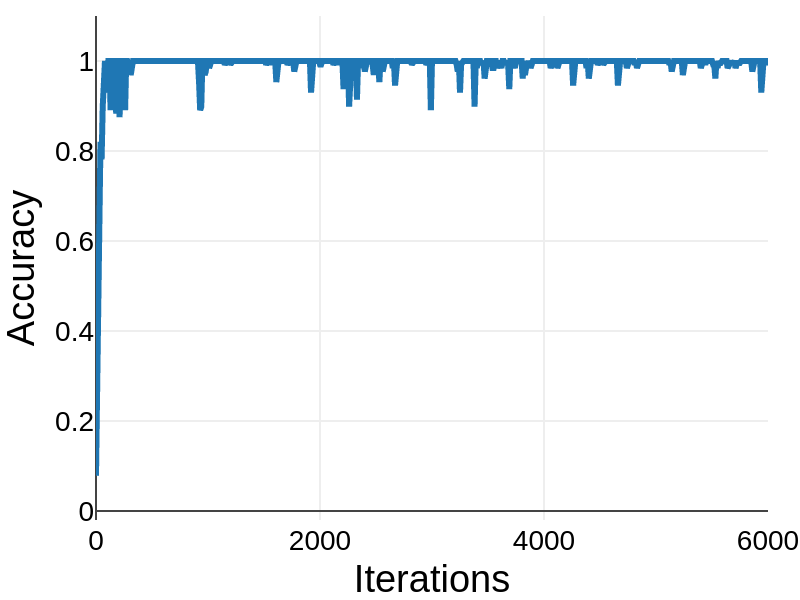
\includegraphics[scale=0.22]{img/rnn-acc-L5}
\caption{}
\end{subfigure}
\begin{subfigure}{0.49\textwidth}
\centering
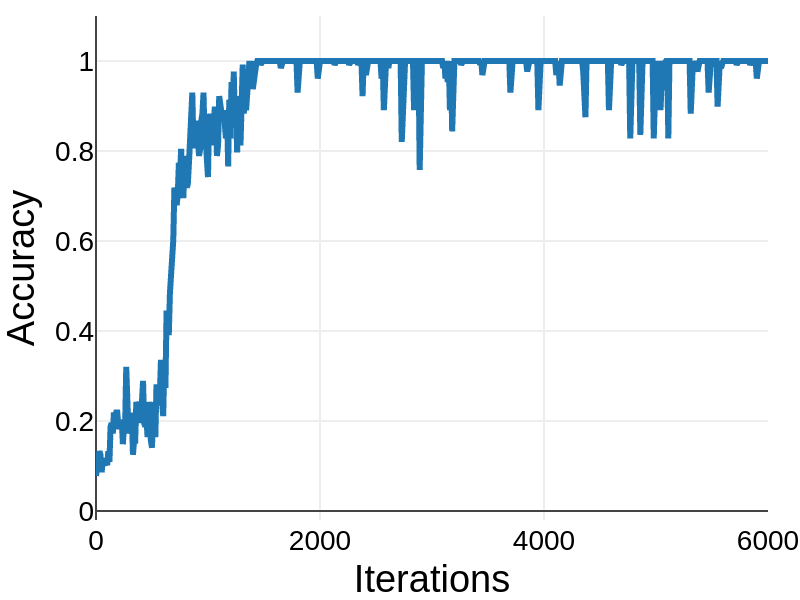
\includegraphics[scale=0.22]{img/rnn-acc-L15}
\caption{}
\end{subfigure}
 \caption{Accuracy curves during training, for sequences of (a) length 5, and (b) length 15. While for a length of 5 the model converges quickly to a high accuracy, longer sequences take longer to converge and the final result is lower.}
\label{fig:rnn_acc_curves}
\end{figure}

\begin{figure}[t]
\centering
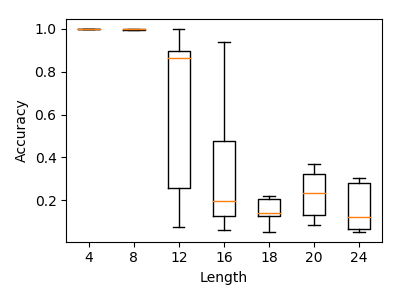
\includegraphics[scale=0.7]{img/rnn-acc-Lbox}
 \caption{Box plots depicting the distribution of the accuracy over 10 runs, for different sequence lengths. As the sequence length increases, obtaining a high accuracy is less likely, and longer sequences tend to random performance.}
\label{fig:rnn_acc_box}
\end{figure}



We run each experiment multiple times as we observed results would vary as sequence length increased

Loss curves for T = 5, 10, 15, 20

Box plots for accuracy of T = 5:20

Show examples of predicted sequences

\bibliographystyle{unsrt}
\bibliography{refs}



\end{document}
